\chapter{Scalable Inference for Discrete-Time Hawkes Processes}
 
Networks capture our intuition about relationships in the world.  They
describe the friendships between Facebook users, interactions in
financial markets, and synapses connecting neurons in the brain.
These networks are richly structured with cliques of friends, sectors
of stocks, and a smorgasbord of cell types that govern how neurons
connect.  Some networks, like social network friendships, can be
directly observed, but in many cases we get but a glimpse of the
network through the actions of its constituents and an understanding
of how the network mediates that activity.  In this work, we focus on
the problem of latent network discovery in the case where the
observable activity takes the form of a mutually-excitatory point
process, also known as a Hawkes process.  We build on previous work
that has taken a Bayesian approach to this problem, specifying prior
distributions over the latent network structure and a likelihood of
observed activity given this network.  We extend this work with a
computationally efficient discrete-time formulation and a stochastic
variational inference (SVI) algorithm that allows us to scale our
approach to long sequences of observations.  We demonstrate our
algorithm on the calcium imaging data used in the Chalearn neural
connectomics challenge.

\section{Introduction}

Networks are abstractions of the relationships and connections between
real-world objects, such as people, stocks, or neurons.  These
connections reflect relationships like ``Wilson and Brady are
friends,'' or ``When neuron A fires it excites neuron B.''  Sometimes
the networks themselves are observed data, as in the case of social
network friendships, but often our view of the network is indirect.
We are left to infer the latent connections between objects based on
our observations of their behavior.  In our neural example, recording
techniques can often provide a measure of the neurons' activity but
cannot resolve the individual synaptic connections between neurons.
Given our knowledge of how synapses work, however, we might infer that
if one neuron consistently fires shortly after another then there is
likely an excitatory connection between them.

This is one example of the \emph{latent network discovery} problem.
We improve upon previous work by providing a discrete-time analogue of
the Hawkes process that is considerably more efficient on datasets
with high rates of activity, and by devising an efficient stochastic
variational inference (SVI) algorithm that can scale to long sequences
of observations.  Most previous work has relied upon Markov chain
Monte Carlo (MCMC) methods for inference, which must consider the
entire observation sequence when evaluating the likelihood of a state,
and which can be prone to poor convergence.  SVI provides an
alternative method of inference that can work with mini-batches (small
subsets) of observations per iteration, and has been shown to yield
dramatic improvements in a variety of large-scale machine learning
problems.

% Hawkes figure
\begin{figure}[t]
  \begin{center}
    % Figure 1a
    \begin{subfigure}[b]{2.34in}
      \caption{Hawkes process dynamics}
      \centering
      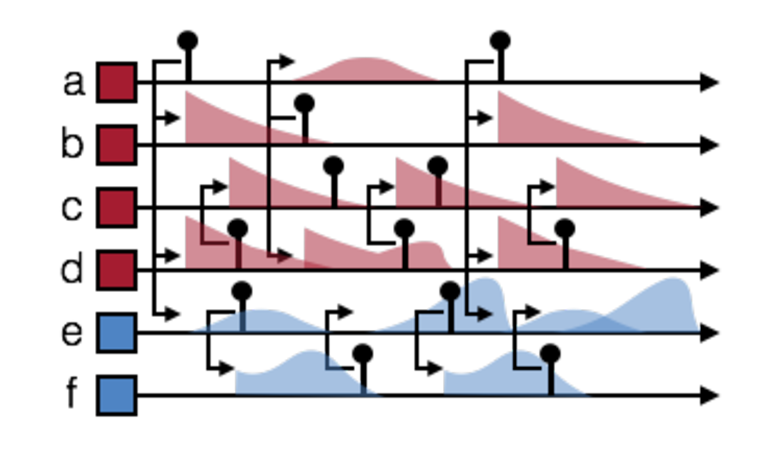
\includegraphics[width=\textwidth]{figures/ch2b/figure1a.pdf} 
      \label{fig:hawkes_a}
    \end{subfigure}
    % Figure 1b
    \begin{subfigure}[b]{0.81in}
      \caption{Weighted Network}
      \centering
      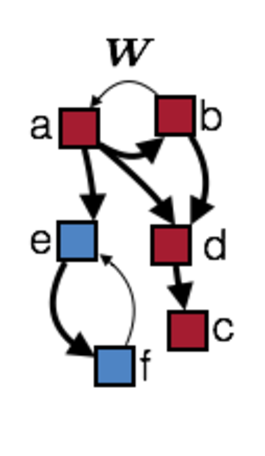
\includegraphics[width=\textwidth]{figures/ch2b/figure1b.pdf} 
      \label{fig:hawkes_b}
    \end{subfigure}
    % Figure 1c
    \begin{subfigure}[b]{2.10in}
      \caption{Impulse responses}
      \centering
      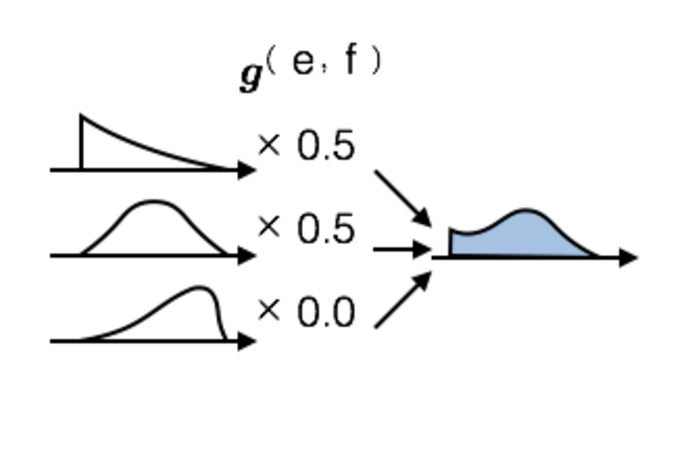
\includegraphics[width=\textwidth]{figures/ch2b/figure1c.pdf} 
      \label{fig:hawkes_c}
    \end{subfigure}
  \end{center}
  % Main caption
  \caption[Components of the discrete time Hawkes process model]{
    Components of the Network Hawkes process model.
    \textbf{(a)} Events induce weighted impulse responses on downstream processes, spawning more events according to the Hawkes process dynamics.
    \textbf{(b)} Underlying these dynamics is a weighted, directed network. Here, the network is a stochastic block model with two clusters of processes (red and blue). Processes primarily connect to others of the same type, though there is a small probability of connection from red to blue.
    \textbf{(c)} We model the impulse responses as a convex combination of normalized basis functions.}
\label{fig:discrete_hawkes}
\end{figure}
% End figure  1

\section{The Discrete Time Network Hawkes Model}
Hawkes processes \cite{Hawkes-1971} are multivariate point processes
that relate excitatory interaction networks to sets of discrete
events.  As with the more familiar Poisson process, the number of
observed events in a particular time window follows a Poisson
distribution, but in a Hawkes process disjoint time intervals are no
longer independent.  This is because the Hawkes process allows events
to influence the future intensity, or rate.  For example, suppose we
have a Hawkes process with two constituent processes.  An event on the
first process could add an \emph{impulse response} to the future rate
of the second process.  More generally, a multivariate Hawkes process
consists of~$N$ individual point processes with
rates~${\{\lambda_n(t)\}_{n=1}^N}$ that depend upon the events that
have occurred up to time~$t$.

Hawkes processes have additive, excitatory interactions.  Each event
adds a nonnegative impulse response to the future rate of connected
processes.  In continuous time, the rate of the~$n$-th process is
\begin{align}
\label{eq:cont_hawkes_rate}
 \lambda_{n}(t) &= \lambda_n^{(0)} + \sum_{m=1}^{M} h_{c_{m} \to n}(t-s_{m}),
\end{align}
where~${\{s_m, c_m\}_{m=1}^{M}}$ is a set of marked spikes where~$s_m
\in [0,T]$ denotes the time of the spike and~${c_m \in \{1, \ldots
  ,N\}}$ is the neuron on which it occurred. The rate is a linear
function of the background rate,~$\lambda_n^{(0)}$, and the impulse
response functions,~${h_{n' \to n}(\Delta t)}$, that govern the
amplitude of influence that events on neuron~$n'$ have on the rate of
neuron~$n$ at time lag~${\Delta t}$. As before, causality and locality
of influence are enforced by limiting the support of the impulse responses
to~$(0, \Delta t_{\mathsf{max}}]$.


The fundamental limitation of the previously developed continuous time
models is that the number of values that the auxiliary
variable~$\omega_m$ can take grows with the number of events which
occurred before time~$s_{m}$. For datasets with high rates of
activity, this can quickly become the limiting factor of the inference
algorithm.  At the same time, it is often reasonable to assume that
events do not interact on time scales faster that~$\Delta t$. This
motivates a discrete time formulation in which we bin events in bins
of width~$\Delta t$ and ignore potential interactions between events
in the same bin. Then the rate becomes,
\begin{align}
\label{eq:disc_hawkes_rate}
\lambda_{t,n} &= \lambda_n^{(0)} +
\sum_{n' = 1}^N \sum_{t'=1}^{t-1} s_{t',n'} \cdot h_{n' \to n}[t-t'], \\
s_{t,n} &\sim \distPoisson(\lambda_{t,n} \cdot \Delta t),
\end{align}
where~$s_{t,n}$ is the number of spikes fired by neuron~$n$ at time~$t$
and~${h_{n' \to n}[t-t']}$ is an impulse response function describing
the influence that events on neuron~$n'$ have on the
rate of process~$n$ at discrete time lag~${t-t'}$. As we will show,
under this formulation the auxiliary variables only assume a fixed set
of values independent of the rate.

In order to incorporate the network model as a prior distribution for
the Hawkes process, we follow the approach of~\citet{Linderman-2014}
and decompose the impulse response function into the product of a
scalar weight that specifies the strength of the interaction and a
probability mass function that specifies the time course of
interaction:
\begin{align*}
  h_{n \to n'}[d]
  &= a_{n \to n'} \cdot w_{n \to n'} \cdot \hbar[d; \, \btheta_{n \to n'}] 
\end{align*}
for~${d \in\{1,\ldots,D\}}$.  

The function~${\hbar[d]: \{1, \ldots, D\} \to
  [0,1]}$ is now a probability mass function.  We model itas a convex
combination of basis functions,~$\bphi_b$, that integrate to one,
\begin{align*}
  \hbar[d; \, \btheta_{n \to n'}]
  &\triangleq \sum_{b=1}^B \theta_{n \to n'}^{(b)} \cdot \phi_b[d], \\
  \sum_{d=1}^D \phi_b[d] \cdot \Delta t  &= 1, \\
  \sum_{b=1}^B \theta_{n \to n'}^{(b)} &= 1.
\end{align*}
We enforce this constraint with a Dirichlet
prior~${\btheta_{n \to n'} \sim \distDirichlet(\bgamma)}$.

Plugging this into~Eq.~\ref{eq:disc_hawkes_rate} yields,
\begin{align*}
  \lambda_{t,n'} &=
  \lambda_{n'}^{(0)} +
  \sum_{n = 1}^N  \sum_{b=1}^B a_{n \to n'} \cdot w_{n \to n'} \cdot 
  \theta_{n \to n'}^{(b)} \sum_{t'=1}^{t-1} s_{t',n} \cdot \phi_b[d] \\
  &=
  \lambda_{n'}^{(0)} +
  \sum_{n' = 1}^N  \sum_{b=1}^B a_{n \to n'} \cdot w_{n \to n'} \cdot
  \theta_{n \to n'}^{(b)} \cdot  \widehat{s}_{t,n,b},
\end{align*}
where
\begin{align*}
  \widehat{s}_{t,n,b} &\triangleq \left(\bs_n \ast \bphi_b\right)[t],
\end{align*}
is the discrete convolution of the~$n$-th spike train with
the~$b$-th basis function evaluated at the~$t$-th time bin.
Since both the spike trains and the basis functions are given,
these can be precomputed.

%Intuitively, the weight~$W_{k\to k'}$ specifies how many child events
%on process~$k'$ will be caused by a single event on process~$k$.
%Then, $G_{k \to k'}[d]$ specifies the probability that the child event
%will occur at lag~$d \Delta t$.  In fact, this procedure is the basis
%of a recursive algorithm for generating samples from the discrete time
%Hawkes process.

Figure~\ref{fig:discrete_hawkes} illustrates the basic components of the model.
We have a stochastic block model with two types of processes (red and
blue) that preferentially interact with processes of the same type.
Events induce weighted impulse responses on downstream processes
according to an underlying latent network (Fig.~\ref{fig:hawkes_b}).
The impulse responses,~${\hbar_{n \to n'}[d]}$, are modeled as a convex
combination of basis functions (Fig~\ref{fig:hawkes_c}).  The impulse
response is weighted according to the strength of the
connection,~$w_{n \to n'}$ before being added to the rate of
downstream processes. \todo{update the figure}

\section{Inference with Gibbs Sampling}

% Discrete vs continuous figure
\begin{figure}{r}{2.5in}
  \centering
  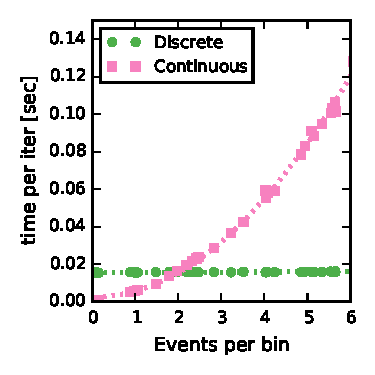
\includegraphics[width=2.5in]{figures/ch2b/discrete_cont_comparison}
  \caption[Runtime comparison of continuous and discrete time Hawkes models]{
    Comparison of run time per Gibbs sweep for the discrete and continuous network Hawkes formulations. Best fit lines added.}
  \label{fig:disc_vs_cont}
\end{figure}

As before, we begin by introducing auxiliary parent variables for each
entry~$s_{t,n}$.  By the superposition theorem for Poisson processes,
each event can be attributed to either the background rate or one of
the impulse responses.

Let~${\omega_{t,n'}^{(n,b)} \in \{0,\ldots, s_{t,n'}\}}$ denote how
many of the events that occurred in the~$t$-th time bin on the~$n'$-th
neuron are attributed to the~$b$-th basis function of the~$n$-th
neuron.  Similarly, let~${\omega_{t,n'}^{(0)}}$ denote the number of
events attributed to the background process. We combine these
auxiliary variables into vectors,~${\bomega_{t,n'}\triangleq
  \left[\omega_{t,n'}^{(0)}, \omega_{t,n'}^{(1,1)}, \ldots,
    \omega_{t,n'}^{(N,B)} \right]}$.

Due to the Poisson superposition principle, these parent variables are
conditionally multinomial distributed.  For time~$t$ and neuron~$n'$,
we resample
\begin{align*}
\bomega_{t,n'} &\sim \distMultinomial \left(s_{t,n'}, \bu_{t,n'} \right) & 
u_{t,n'}^{(0)} &= \frac{\lambda_{0,n'}[t]}{\lambda_{n'}[t]}, &
u_{t,n'}^{(n,b)} &= \frac{\hat{s}_{t,n,b} \cdot a_{n \to n'} \cdot w_{n \to n'} \cdot \theta_{n \to n'}^{(b)}}{\lambda_{n'}[t]}\, .
\end{align*}
Given this attribution, the likelihood factorizes into a product of
Poisson distributions,
\begin{multline*}
  p(\bomega \given \blambda) =
  \left[\prod_{t=1}^T \prod_{n'=1}^N \distPoisson(\omega_{t,n'}^{(0)} \given \lambda_{n'}^{(0)} \Delta t)\right]  \\
  \times
  \left[ \prod_{t=1}^T \prod_{n=1}^N \prod_{n'=1}^N \prod_{b=1}^B
    \distPoisson(\omega_{t,n'}^{(n,b)} \given
    \hat{s}_{t,n,b} \cdot a_{n \to n'} \cdot w_{n \to n'} \cdot \theta_{n\to n'}^{(b)} \cdot \Delta t)\right].
\end{multline*}

\paragraph{Gibbs sampling the background rates.}
We use conjugate priors for the constant background rates, weights,
and impulse responses.  For the constant background rates we have,
${\lambda_{n'}^{(0)} \sim\distGamma(\alpha_\lambda, \beta_\lambda)}$,
which results in the conditional distribution
\begin{align*}
\lambda_{n'}^{(0)} \given \{\omega_{t,n'}^{(0)}\} &\sim
\distGamma(\alpha_\lambda^{(n)}, \beta_\lambda^{(n)}), \\
\alpha_\lambda^{(n)} &= \alpha_\lambda + \sum_{t=1}^T \omega_{t,n'}^{(0)}, \\
\beta_\lambda^{(n)} &= \beta_\lambda + T \Delta t\,.
\end{align*}

\paragraph{Gibbs sampling impulse responses.}
The likelihood of the impulse responses,~$\btheta_{n \to n'}$ is
proportional to a Dirichlet distribution.  Combined with
a~$\text{Dirichlet}(\bgamma)$ prior this yields
\begin{align*}
  \btheta_{n \to n'} \given \{\omega_{t,n}^{(n',b)}\}, \bgamma
  &\sim \distDirichlet\left( \bgamma_{n \to n'} \right), \\
  \gamma_{n \to n'}^{(b)} &=  \gamma_b + \sum_{t=1}^T \omega_{t,n'}^{(n, b)}\,.
\end{align*}

\paragraph{Gibbs sampling the weighted adjacency matrix.}
As before, the weights are conjugate with a gamma
prior,~$\distGamma(\kappa, \nu)$.  Given the adjacency matrix~$\bA$
and the auxiliary parent variables, the conditional distribution is,
\begin{align*}
  w_{n \to n'} \given a_{n \to n'}\!=\!1
  &\sim \distGamma(\kappa^{(n,n')}, \nu^{(n,n')}), \\
  \kappa^{(n,n')} &= \kappa +\! \sum_{t=1}^T \sum_{b=1}^B \omega_{t,n'}^{(n,b)}, \\
  \nu^{(n,n')} &= \nu +\! \sum_{t=1}^T s_{t,n}.
\end{align*}
As in the previous chapter, in order to resample~$\bA$, we iterate over
each entry and sample from the marginal distribution after integrating
out the parents. We assume the parameters of the network prior can be
sampled efficiently -- a reasonable assumption for many random network
models.

The continuous time representation introduces a latent ``parent''
variable for each event in the dataset, and the parent can be any one
of the events that occurred in the preceding window of influence. Call
the number of potential parents~$M$. The discrete time representation
has a multinomial r.v. for each time bin that contains at least one
event, and the support of this multinomial is always a fixed
size,~${NB+1}$.  When the rate of events is high, $NB+1 \ll M$,
allowing for dramatic improvements in efficiency in the discrete case.

Figure~\ref{fig:disc_vs_cont} shows the time per full Gibbs sweep as a
function of the number of events per discrete time bin for the
discrete and continuous formulations. The discrete formulation incurs
a constant penalty whereas the continuous formulation quickly grows
with the event rate. For low rates, the continuous formulation can be
advantageous, but the discrete model is vastly superior in many
realistic settings. For example, Linderman and Adams worked with
trades on the S\&P100, which occur tens or hundreds of times per
second for each stock. Since the complexity of their algorithm grows
with the number of events, they down-sampled the data to consider only
the times when a stock price significantly changed.

\section{Stochastic Variational Inference}
The discrete time formulation offers advantageous complexity compared
to the continuous analogue, but it still must resample the entire set
of parents each iteration in order to maintain the invariance of the
posterior distribution. In many cases, a mini-batch of time bins can
provide substantial information about the global parameters of the
model, and rapid progress can be made by iterating quickly over
subsets of the data. This motivates our derivation of a stochastic
variational inference (SVI) algorithm for the network Hawkes process.

Variational methods optimize a lower bound on the marginal likelihood
by minimizing the KL-divergence between a tractable approximating
distribution and the true posterior. Since the data-local parents
variables are conditionally independent given the global
parameters~($\bW$,~$\btheta$,~etc.), our variational approach will
easily extend to the stochastic setting in which we compute unbiased
estimates of the gradient of the variational objective using
mini-batches of data.

The primary impediment to deriving a variational approximation is the
nonconjugacy of the spike-and-slab prior on the weights.  To overcome
this, we approximate the spike-and-slab prior with a mixture of gamma
distributions, as has previously explored by~\citet{Grabska-2013}:
\begin{align*}
q(a_{n \to n'}) &= \distBernoulli(a_{n \to n'} \given \widetilde{p}_{n \to n'}), \\
q(w_{n \to n'} \given a_{n \to n'}) &=
\begin{cases} 
\distGamma(w_{n \to n'} \given \widetilde{\kappa}_1^{(n, n')}, \widetilde{\nu}_1^{(n,n')}, a_{n \to n'} =1), \\
\distGamma(w_{n \to n'} \given \widetilde{\kappa}_0^{(n, n')}, \widetilde{\nu}_0^{(n, n')}, a_{n \to n'} =0)\,.
\end{cases}
\end{align*}
As~$\kappa_0 \to 0$ and~$v_0\to \infty$, the gamma distribution
approaches a spike at zero.

We use a fully-factorized variational approximation except for a joint
factor for each connection,~$a_{n\to n'}$ and $w_{n \to n'}$.  Since
the model is fully conjugate, the factors are easily derived.

% Parents
\paragraph{Variational updates for parent variables,~$q(\bomega_{t, n'})$} 
For the parent variables, the variational updates are
\begin{align*}
q(\bomega_{t,n'}) &= \distMultinomial(\bomega_{t, n'} \given s_{t,n'}, \widetilde{\bu}_{t,n'}), \\
\widetilde{u}_{t,n'}^{(0)} &= \frac{1}{Z} \exp\left\{\mathbb{E}_{\blambda}[\ln \lambda_{n'}^{(0)}]\right\}, \\
\widetilde{u}_{t,n'}^{(n,b)} &= \frac{1}{Z} \hat{s}_{t,n,b} \exp\left\{\mathbb{E}_{\btheta} [\ln \theta_{n \to n'}^{(b)}] + \mathbb{E}_W[\ln w_{n \to n'}]\right\},
\end{align*}
where~$Z$ is the normalization constant.

% Background rates
\paragraph{Variational updates for background rates,~$q(\lambda_n^0)$}
The variational form parameters of the gamma distribution over
background rates are
\begin{align*}
q(\lambda_n^0) &= \distGamma(\lambda_n^{0} \given \widetilde{\alpha}_{\lambda}^{(n)}, \widetilde{\beta}_{\lambda}^{(n)}),  \\
\widetilde{\alpha}_{\lambda}^{(n)} &= \alpha_\lambda + \sum_{t=1}^T \mathbb{E}_{\bomega}\left[ \omega_{t,n}^{(0)}\right], \\
\widetilde{\beta}_{\lambda}^{(n)} &= \beta_\lambda + T \Delta t\,.
\end{align*}


% Impulse response parameters
\paragraph{Variational approximation for impulse response parameters,~$q(\btheta_{n \to n'})$}
With the conjugate prior formulation the variational parameter updates
for the Dirichlet distributed impulse response parameters are
\begin{align*}
q(\btheta_{n \to n'}) &= \distDirichlet(\bn_{n \to n'} \given \widetilde{\bgamma}^{(n,n')}), \\
\widetilde{\gamma}_b^{(n,n')} &= \gamma_{b} + \sum_{t=1}^T \mathbb{E}_{\bomega}\left[\omega_{t,n'}^{(n,b)}\right]\,.
\end{align*}

% Weights and adjacent matrix
\paragraph{Variational approximation for the weighted adjacency matrix.}
The primary motivation for adopting a weakly sparse mixture of gamma
distributions is to derive an efficient variational inference
algorithm.  The mixture-of-gammas prior is conjugate with the Poisson
observations, and hence the variational distribution is also a mixture
of gammas:
\begin{align*}
  q(w_{n \to n'} \given a_{n \to n'}=1)
  &= \distGamma(w_{n \to n'} \given
  \widetilde{\kappa}^{(n,n')}_1,
  \widetilde{\nu}^{(n,n')}_1) \\
  \widetilde{\kappa}^{(k,k')}_1
  &= \kappa + \sum_{t=1}^T \sum_{b=1}^B \mathbb{E}_{\bomega}\left[\omega_{t,n'}^{(n,b)}\right] \\
  \widetilde{\nu}^{(n,n')}_1
  &= \nu + \sum_{t=1}^T s_{t,n}\,,
\end{align*}
and likewise for the ``spike'' factor,
\begin{align*}
  q(w_{n \to n'} \given a_{n \to n'}=0)
  &= \distGamma(w_{n \to n'} \given
  \widetilde{\kappa}^{(n,n')}_0,
  \widetilde{\nu}^{(n,n')}_0) \\
  \widetilde{\kappa}^{(k,k')}_0
  &= \kappa_0 + \sum_{t=1}^T \sum_{b=1}^B \mathbb{E}_{\bomega}\left[\omega_{t,n'}^{(n,b)}\right] \\
  \widetilde{\nu}^{(n,n')}_0
  &= \nu_0 + \sum_{t=1}^T s_{t,n}\,,
\end{align*}

% Adjacency matrix
This leaves us with~$q(a_{n \to n'})$, which is Bernoulli distributed
with parameter~$\widetilde{p}_{n \to n'}$.  Collecting all the terms
that include~$A_{n \to n'}$ and lack~$w_{n \to n'}$ yields
\begin{multline*}
 \frac{\widetilde{p}_{n \to n'}}{1-\widetilde{p}_{n \to n'}} =  \\
 \frac{\exp\{\mathbb{E} [\ln p] \} }{\exp\{\mathbb{E}[\ln (1-p)] \}} \times 
\frac{ (\exp\{\mathbb{E} [\ln \nu] \})^{\kappa} }{ \Gamma(\kappa)} \times 
\frac{\Gamma(\widetilde{\kappa}^{(n,n')}_1)}{ (\widetilde{\nu}^{(n,n')}_1)^{\widetilde{\kappa}^{(n,n')}_1} } \times
\frac{\Gamma(\kappa_0)}{ (\nu_0)^{\kappa_0} } \times
\frac{(\widetilde{\nu}^{(n,n')}_0)^{\widetilde{\kappa}^{(n,n')}_0}}{ \Gamma(\widetilde{\kappa}^{(n,n')}_0)}\,.
\end{multline*}

% network model
As with Gibbs sampling, we assume a variational approximation for the network model can be derived, and provide access to the necessary expectations,~$\mathbb{E}[\ln p]$, $\mathbb{E}[\ln(1-p)]$,~$\mathbb{E}[\nu]$ and~$\mathbb{E}[\ln \nu]$. 

As aforementioned, the time bin are conditionally independent given the network weights and the adjacency matrix -- a common pattern exploited by stochastic variational inference (SVI) algorithms \cite{Hoffman-2013}.
These methods optimize the variational objective using stochastic gradient methods that work with mini-batches of data.
Often, a mini-batch of data can provide valuable information about the global parameters, in our case the network and background rates. 
Quickly iterating over these global parameters allows us to reach good modes of the posterior distribution in a fraction of the time that standard variational Bayes and Gibbs sampling require, since those methods must process the entire dataset before making an update.
SVI does require some tuning, however. In particular, we must set a mini-batch size and a step size schedule.
In this work, we fix the mini-batch size to~${T_{\mathsf{mb}}=1024}$ and set the  step size at iteration~$i$ to~${(i+1)^{-0.5}}$.
These parameters may be  tuned with general purpose hyperparameter optimization techniques \cite{Snoek-2012}.

%% Synthetic Results 
\section{Synthetic Results}

% Predictive log likelihood vs run time (Short dataset)
\begin{figure}[t!]
  \begin{center}
    % Short dataset
    \begin{subfigure}[b]{0.48\linewidth}
      \caption{Short dataset: $T=10^4$}
      \centering
      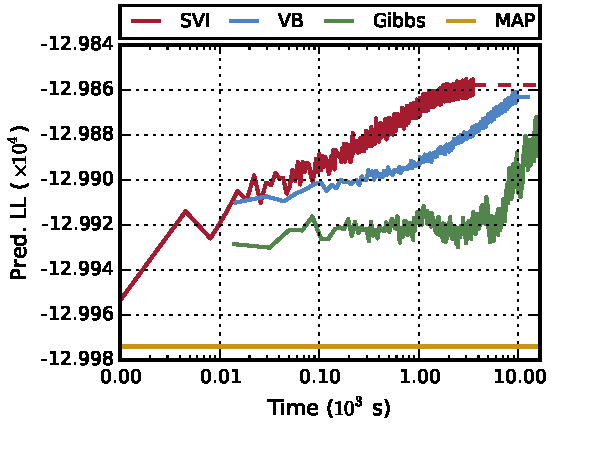
\includegraphics[width=2.625in]{figures/ch2b/figure2a.pdf} 
      \label{fig:synth_pll_short}
    \end{subfigure}
    ~
    % Longer dataset
    \begin{subfigure}[b]{0.48\linewidth}
      \caption{Long dataset: $T=10^5$}
      \centering
      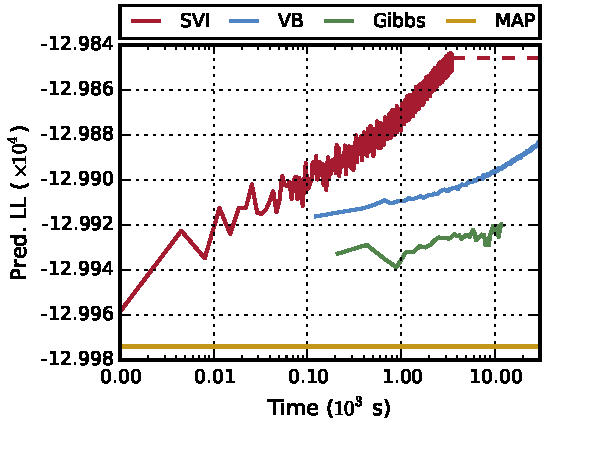
\includegraphics[width=2.625in]{figures/ch2b/figure2b.pdf} 
      \label{fig:synth_pll_long}
    \end{subfigure}
    %
    \caption[Predictive log likelihood versus wall clock time]{
      Predictive log likelihood versus wall clock time for three Bayesian inference algorithms on a dataset of~$K=50$ processes and~$T=10^4$ and~$T=10^5$ time bins on the left and right, respectively.}
    \label{fig:synth_pll}
  \end{center}
\end{figure}


We assess the performance of the proposed inference algorithms on a synthetic dataset generated by a strongly sparse Hawkes process with~${K=50}$ processes.
We used a stochastic block model network prior with~${C=5}$ clusters, each consisting of ten densely connected processes~(${p_{c\to c}=0.4}$), with sparse connections to processes in other clusters~(${p_{c\to c'}=0.01}$).
All weights share the same scale of~$v=5.0$, though this information is not provided \emph{a priori}.
We simulate~${T=10^5}$ time bins in steps of size~${\Delta t=1}$.
The processes have an mean background rate of~$1.0$ event per time bin and, due to the network interactions, the average total rate of the processes is~$16.7 \pm 12.0$ events per bin.
Referring to Figure~\ref{fig:disc_vs_cont}, this is a regime that favors the discrete model.
We initialized by performing MAP estimation on the first~$T_{\mathsf{init}}=10^4$.
Then we trained the model using Gibbs sampling, batch variational Bayesian inference (VB), and stochastic variational inference (SVI) 

We trained the models on only the first~$10^4$ time bins, the same that were used for initialization.
We evaluated the algorithms in terms of their predictive log likelihood on a held-out dataset of length~$T_{\mathsf{test}}=10^3$.
Figure~\ref{fig:synth_pll_short} shows the results as a function of wall-clock time.
We find that SVI obtains competitive predictive log likelihood in a matter of minutes.
Batch VB and Gibbs converge at a considerably slower rate, though they eventually match the SVI predictive likelihood after hours of computation.
The MAP estimate, even with cross validated regularization, underperforms the other competing algorithms.

This trend is amplified when we consider the entire training set of size~$T=10^5$.
Figure~\ref{fig:synth_pll_long} illustrates the power of SVI in handling these large time datasets.
Considerable information about the global parameters (e.g., the network) can be gained from just a mini-batch of time points.
Hence, we can make rapid improvements in predictive log likelihood very quickly.
By contrast, each step of the Gibbs and batch VB algorithms is approximately 10 times slower, and even after computing sufficient statistics over the entire dataset, the algorithm is only able to make limited progress per iteration.

% Some results on a connectomics dataset
\section{Connectomics Results}

% Connectomics results
\begin{figure}[t!]
  \begin{center}
    % a. the data
    \begin{subfigure}[b]{0.32\linewidth}
      \caption{}
      \centering
      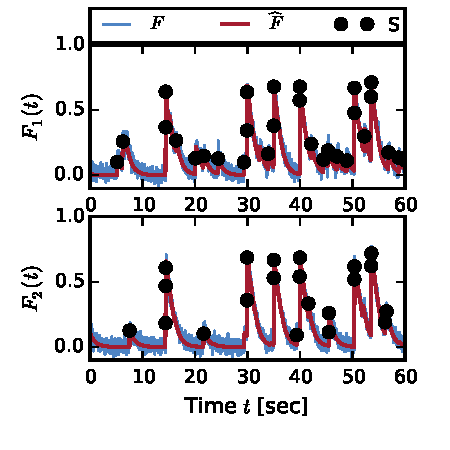
\includegraphics[width=\textwidth]{figures/ch2b/figure3a.pdf} 
      \label{fig:connectomics_data}
    \end{subfigure}
    % b. True network with block structure
    ~
    % c. ROC
    \begin{subfigure}[b]{0.32\linewidth}
      \caption{}
      \centering
      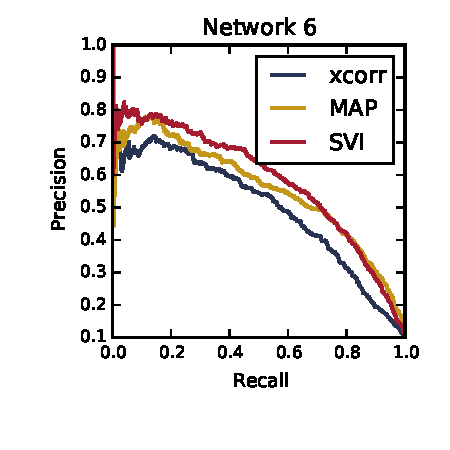
\includegraphics[width=\textwidth]{figures/ch2b/figure3d.pdf} 
      \label{fig:connectomics_prc}
    \end{subfigure}
    ~
    % d. Precision Recall
    \begin{subfigure}[b]{0.32\linewidth}
      \caption{}
      \centering
      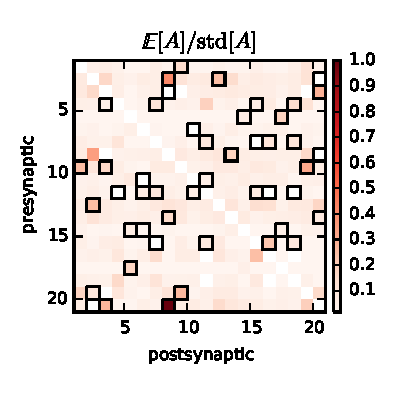
\includegraphics[width=\textwidth]{figures/ch2b/chalearn_confidence.pdf} 
      \label{fig:connectomics_zscore}
    \end{subfigure}
    % Main caption
    \caption[Discrete time Hawkes process applied to connectomics challenge]{
      Application of the network Hawkes model to a connectomics challenge.
      \textbf{(a)} The data is in the form of a calcium fluorescence trace, which we preprocess to extract neural spike times.
      \textbf{(b)} We measure performance on a link prediction task using a precision-recall curve and find that the posterior estimates of SVI provide the best estimates on some networks. In addition to an estimate of the connection probability and weight, SVI provides an estimate of the posterior uncertainty.
      \textbf{(c)} Inferred $\mathbb{E}_q[\bA] / \text{std}_q[\bA]$ for the first 20 neurons. True connections are outlined in black.}
    \label{fig:connectomics}
  \end{center}
\end{figure}

We tested these inference algorithms on the data from the Chalearn neural connectomics challenge\footnote{\url{http://connectomics.chalearn.org}} \cite{Stetter-2012}.
The data consist of calcium fluorescence traces,~$\bF$, from six networks of~$K=100$ neurons each. We use ten minutes of data at 50Hz sampling frequency to yield~$T=3\times 10^6$ entries in~$\bS$.
In this case, the networks are purely excitatory, and each action potential, or spike, increases the probability of the downstream neurons firing as a result.
This matches the underlying intuition of the Hawkes process model, making it a natural choice.  

In order to apply the Hawkes model, we first convert the fluorescence traces into a spike count matrix using OOPSI, a Bayesian inference algorithm based on a model of calcium fluorescence \cite{Vogelstein-2010}.
The output is a filtered fluorescence trace,~$\widehat{\bF}$, and a probability of spike for each time bin.
We threshold this at probability~$0.7$ to get a~$T\times K$ binary spike matrix,~$\bs$.
This preprocessing is shown in Figure~\ref{fig:connectomics_data}.

Figure~\ref{fig:connectomics_prc} shows the precision-recall curve we used to evaluate the algorithms' performance on network recovery. As a baseline, we compare against simple thresholding of the cross correlation matrix. On Network 6, SVI offers the best network inference. Table 5 shows the results on the other five networks using the same model parameters. On 4/5 of these networks, the Bayesian methods offer the best performance. 

Figure~\ref{fig:connectomics_zscore} illustrates one of the main advantages of the fully Bayesian inference algorithm -- calibrated estimates of posterior uncertainty. Here we show the SVI algorithm's estimate of the posterior mean of~$\bA$ normalized by the posterior standard deviation for a subset of 20 neurons from Network 6. We also outline the true connections to show that the most confident predictions are more likely to correspond to true connections. Such estimates of the posterior uncertainty are not available with standard heuristic methods or point estimates.

% A fancy table with results for each of the networks
\begin{table}
  \centering
  \resizebox{\textwidth}{!}{%
    \begin{tabular}{ c||c|c||c|c||c|c||c|c||c|c }
      %\hline
      %\multirow{3}{*} \textbf{Algorithm} 
      & \multicolumn{2}{c||}{Network 1}
      & \multicolumn{2}{c||}{Network 2}
      & \multicolumn{2}{c||}{Network 3}
      & \multicolumn{2}{c||}{Network 4}
      & \multicolumn{2}{c}{Network 5} \\
      \cline{2-11}
      Algorithm
      & ROC & PRC
      & ROC & PRC
      & ROC & PRC
      & ROC & PRC
      & ROC & PRC \\
      %\hhline{=#=|=#=|=#=|=#=|=#=|=}
      \hline
      xcorr & 0.596 & 0.139 & 0.591 & 0.133 & \bf{0.701} & \bf{0.198} & 0.745 & 0.296 & 0.798 & 0.359  \\
      \hline
      MAP & 0.607 & 0.174 & \bf{0.619} & \bf{0.143} & 0.698 & 0.178 & \bf{0.790} & 0.334 & \bf{0.859} & 0.408 \\
      \hline
      SVI  & \bf{0.649} & \bf{0.184} & 0.605 & 0.141  & 0.673 & 0.176 & 0.774 & \bf{0.342}  & 0.844 & \bf{0.410}\\
      \hline
    \end{tabular}
  }
  \caption[Comparison of inference algorithms on the Chalearn connectomics challenge]{Comparison of inference algorithms on link prediction for five networks from the Chalearn connectomics challenge. Performance is measured by area under the ROC curve and area under the precision recall curve (PRC). In four of the five networks a Hawkes process model provides the best results.}
\end{table}

\begin{comment}
\section{Related Work}
The Hawkes process is closely related to the generalized linear model (GLM) with Poisson observations, which is widely used in computational neuroscience \cite{Paninski-2004, Pillow-2008}.  
In fact, the Hawkes process is a special case of the Poisson GLM in which the link function is linear and the impulse responses are non-negative. 
As in the Poisson GLM, the negative log likelihood of the Hawkes process is convex enabling efficient maximum likelihood and maximum a posteriori estimation. 
The advantage of the Hawkes process is that its linear form allows for elegant fully Bayesian inference -- a task which is non-trivial  in the Poisson GLM due to the lack of conjugacy. With these Bayesian inference algorithms, we can estimate and reason under the posterior uncertainty of the model.

One of the earliest applications of Hawkes processes in machine
learning was the work of~\citet{Simma-2010}, which developed an
expectation-maximization algorithm based upon the auxiliary variable
parent formulation. Observing that~$\lambda_{k}(t)$ is a sum of
impulse responses, \citet{Simma-2010} invoked the Poisson
superposition principle to motivate a set of auxiliary ``parent''
variables,~$z_{k,n}$, which denote the origin of the~$n$-th event on
process~$k$, either the background rate or an impulse response from a
previous event. Conditioned upon these auxiliary variables, the
likelihood factorizes over impulse responses.

%\TODO{reference Iwata and Zhou -- stochastic EM, convex optimization}
Subsequent works leveraged this intuition to extend Hawkes processes with interpretable prior distributions over the network of impulse responses.
\citet{Blundell-2012} introduced an infinite relational model prior over the network of interactions as well as a Gibbs sampling algorithm for fully Bayesian inference.
\citet{Dubois-2013} explored the use of infinite relational models as a prior in conjunction with a point process observation model build on a Gibbs sampling algorithm.
Recently,~\citet{Linderman-2014} developed a general framework for combining random ``spike-and-slab'' network models with Hawkes processes that uses a continuous time formulation and an auxiliary Gibbs sampling inference algorithm.
\citet{Guo-2014} have developed a similar model that focuses on applying Hawkes processes to language modeling and incorporating features of the discrete events.

We extend the work of \citet{Linderman-2014} by addressing two shortcomings: the limited scalability of the continuous time formulation which introduces auxiliary variables for each event in the dataset, and the batch nature of their Gibbs sampling algorithm. We address the former by deriving a discrete time version of their model which vastly outperforms the continuous time version on datasets with high rates of activity. To overcome the batch nature of the Gibbs algorithm, we make an approximation to the spike-and-slab network model that renders the model fully conjugate, thereby enabling efficient stochastic variational inference \cite{Hoffman-2013} on mini-batches of data.
\end{comment}

\section{Conclusion}
We presented a scalable stochastic variational inference algorithm for the problem of Bayesian network discovery with Hawkes process observations. Building on previous modeling work, we leveraged a weak sparsity model to obtain a fully conjugate model. We focused on scaling to long duration recordings (large~$T$). Scaling to large networks (large~$K$) is nontrivial due to dependencies among weights, but in future work we hope to explore approximate algorithms to tackle this important problem.
